\documentclass[12pt]{article}
\usepackage[english]{babel}
\usepackage[utf8x]{inputenc}
\usepackage{amsmath}
\usepackage{graphicx}
\usepackage{setspace} 
\usepackage{natbib}
\usepackage{float}
\usepackage[top=1in, bottom=1in, left=1.5in, right=1.5in]{geometry}


\title{Historical Geographies of Diabetes and Emotion}
\author{gENTRY hANKS}
\begin{document}
\maketitle


%\newpage
%\begin{abstract}
%\singlespacing 
%\end{abstract}

\newpage
\section{How Is This Geographical?}
\doublespacing
Turning to David \citet{livingstone_geographical_1993} and embracing his approach to ``The Geographical Tradition,'' I employ his questions ``What role, for example, did geography play in past society? Was it used for political, or religious or economic purposes by particular groups? Who benefited from the latest theory, and who lost out?'' (p. 2).  With these questions in mind, Firstly I bring to the fore an overview of different perspectives on diabetes from different places and pieces of history, then provide an examination of medical literature, historical writings and archival material to geographically situate the social, political and economic contexts of historical scientific thought on diabetes in relation to emotion, which will include historical examples of what role emotion plays and how it has been understood throughout a history of diabetes. \citet{livingstone_geographical_1993} warns, ``reconstructing intellectual history is never a once-and-for-all activity'' (p. 3), but allows one to ``work with a more realistic picture of geograhical knowledge as a cultural product and a political resource, without assuming that scientific knowledge is somehow immune to such forces'' (p. 3). There are limitations to this historical approach beginning with the fact that ``the past...is only contemplated in terms of the present'' \citep[p. 3]{livingstone_geographical_1993}. There is also the business of selection, because ``inevitably historians are involved in selecting from the available sources the material they deem significant in light of the problems under scrutiny'' (p. 4), I will be unable to tell a whole or complete story where facts are somehow able to represent themselves, but instead, ``the historian stage-manages their performance on the contemporary scene'' \citep[p. 5]{livingstone_geographical_1993}. 








I put forth that, over time and place, different geographical locations within the body have come to be understood as the ``seat'' of the illness.  For this analysis I will rely on literature review and Archival methods. Archival materials are a staple of historical geography and they like geography have a sorted history with colonialsism and power. 

\section{Background}
\doublespacing
Mainstream historical accounts of diabetes are well documented \citep{engelhardt_diabetes_1989, tattersall_diabetes_2009}, but are often too quick to fast forward to the discovery of insulin. There have descriptions of the symptoms of diabetes at least as old as the 11th centry BCE when Susruta, an Indian physician, documented the condition, which didn't receive this name until Greek physician, Aretaeus in 100 BCE. He used the Greek word, \textit {dia-bainein} meaning ``to siphon'' \citep{sattley_history_1996}.  

Up until the Renaissance, the medical writings of prolific Greek scholar and physician Claudius Galen (130--201 BCE) were seen as doctrine not only in European medicine, but were also regarded in the medical practices of Persia and Arabia \citep{henschen_1969_term}. Galen wrote about the seat of the illness (diabetes), that is, where the disease was geographically located as indicated by organ names. He described diabetes as a type of dropsy and gave rise to a long held misbelief that the kidneys were responsible for the symptoms of diabetes \citep{henschen_1969_term}. 

Using divisions from medical historians as provided by \citet{sanders_2001_philatelic} will prove useful in organizing some background information on diabetes. Sanders warns the reader at the beginning of his book that there is no way to provide a complete or whole history and ``the omission of any event or individual's role in the history of diabetes in no way lessens the importance of that contribution'' (p. xiii). 
\citet{sanders_2001_philatelic} names the 4 divisions of the history of diabetes, ``The Descriptive Period: describing and naming the disease, The Diagnostic Period: learning how to diagnose the disease, The Experimental Period: learning what causes the disease and the Therapeutic Era: learning how to treat the disease.'' (p. 1), which are well accepted by medical hisotrians \citep{papaspyros_1964_history}. Sanders has also offered a fifth period, ``The Era of Complications, in which we learn how diabetes causes additional health problems'' (p. 1). These periods are not discrete as there are temporal and geographical overlaps. For example, 2000 years before Hippocrates, physicians in Egypt had already described diabetes and were already seeking ways to diagnose and treat the condition \citep{sanders_2001_philatelic}. 

\subsection{Describing Diabetes}

Egyptian physicians produced 7 papyri from 2000 BCE to 1200 BCE, one of particular interest-- The Ebers \citep{bryan_1974_ancient}. The Ebers Papyrus was written circa 1550 BCE and describes polyuria (frequent urination that causes dehydration and extreme weight loss) and remedies for polyuria \citep{bryan_1974_ancient}. 
While Hippocrates (460-- 377 BCE), perhaps the most widely recognized Greek Physician, didn't write about diabetes specifically, he too described conditions of extreme urination and body wasting \citep{avicenna_1930_treatise}. 

Another Greek physician, Aretaeus (130--200 CE), who was mentored by Hippocrates and a coeval of Galen, hailed from Cappadocia, which is in modern day Turkey \citep{henschen_1969_term}. As mentioned earlier, Aretaeus is credited with using the term diabetes to describe the body as a siphon through which liquids entered and then were quickly dispelled. Aretaeus, like Galen, believed that the source of diabetes was located in the kidneys. He also believed it to be a disease of the bladder. According to \citet{aretaeus_1856_extant},
``for the thirst there is need for a powerful remedy, for in kind it is the greatest of all sufferings; and when fluid is drunk, it stimulates the discharge of urine; and sometimes as it flows off it melts and carries away with it the particles of the body'' (p. 487).  This liquification of the flesh into urine is used to describe diabetes in quite a few historical medical accounts. ALthough he isn't the first to describe the pancreas, Rufus of Ephesus \footnote {The exact origin of the term is not known and contested \citep{sanders_2001_philatelic}.} is credited with coining the term \textit{pancreas} (c. 100 CE): \textit{pan} meaning all and \textit{kreas} meaning flesh due to the organ's perceieved amorphous shape \citep{papaspyros_1964_history}. 

Although Hindu medical writings described urine from a person with diabetes as honeyed well before Europeans \citep{frank_1957_diabetes}, 
Western historians place emphasis on the Latin term \textit{mellitus}, which then allows the West to claim linguistic authority over medical knowledge. The Vedic Scriptures in Sanskrit provided the basis of Hindu medical knowledge, which came to be a set of three medical textbooks known as \textit{samhitas} and were named for 3 renowned hindu physicians-- Chakara, Susruta and Vagbhata \citep{frank_1957_diabetes}. These texts are believed to have been written between 100 BCE and 700 CE.  Many European physcians of the ancient world mistakenly identified the residue left from evaporated urine of PWD as salt instead of sugar. Hindu medicine primarily focused on prevention of diabetes and very little on the treatment of the symptoms \citep{frank_1957_diabetes}. The treatments they did implement were unfortunately diets high in carbohydrates and emetics along with the helpful suggestion of weight reduction and plenty of exercise \citep{sanders_2001_philatelic}. The medical writings of Chakara and Vagbhata offer 20 varieties of diseased urine or urination known as \textit{prameha}, one of which Chakara describes the patient as losing strength, then flesh and finally the loss of a healthy complexion \citep{frank_1957_diabetes}. While Chakara and Susruta briefly mention that insects are attracted to the urine of PWD, the writings of Vagbhata provide more detail about how diabetes is acquired, which is of importance in a medical system that focuses on prevention. \textit{Prameha} was described by Hindu physicians as having the potential to be inherited or acquired and displaying characteristics \citep{frank_1957_diabetes} such as extreme thirst, obesity, chronic fatigue, obesity, recurring infections, impotence and excessive urination in both frequency and quantity \citep{frank_1957_diabetes}. 

In 3rd century BCE China, a dialogue between the Yellow Emperor and his personal minister was written and came to be widely known as the \textit{Nei Ching} and was revised in the 8th century CE \citep{veith_1950_huang}. The \textit{Nei Ching}, beleived to be written by Huang Ti (The Yellow Emporer), is the foundation of Chinese and Japanese traditional medicine and like Hindu medicine was also prevention focused. Symptoms like insatiable thirst and abnormally frequent and copious urination make an appearance in the \textit{Nei Ching} \citep{veith_1950_huang}. 

After the demise of the Roman Empire, during the middle ages of Europe, medical concepts were based in the writings of Hippocrates and relied on understanding the four humors-- blood, phlegm, yellow bile and black bile \citep{lloyd_1983_hippocratic}. The middle ages, for the most part, aren't known for their advances in physiology and anatomy. This vacuum of knowledge led to a robust desire to understand the composition of the human body in the centuries to come \citep{sanders_2001_philatelic}. 

During the 11th and 12th centuries two prolific physicians, Avicenna from Persia and Maimonides of Arabia, proffered new knowledge about diabetes. Avicenna (Ibn Sina) was a philosopher and physician who attempted to compile as much medical knowledge of his time into a medical textbook-- the \textit{Qanun}, which was originally written in Persian and translated into Latin in the 12th century \citep{avicenna_1930_treatise}. Avicenna was held in such high regard that he was often reffered to as Galen's equal \citep{sanders_2001_philatelic}. In the \textit{Qanun} (The \textit{Canon of Medicine}) Avicenna gave detailed accounts of tasting sweet urine, unyielding wounds, diabetic gangrene, and withering bodies, as well as and understanding that diabetes could either be primary or secondary \citep{avicenna_1930_treatise}. 

Islamic beleifs were incongruent with the practice of cadaver dissection, causing Avicenna to be somewhat lacking in his knowledge of human anatomy and giving way to his heavily philosophical understandings of medicine. Human cadaver dissection was a rare practice in Greek antiquity \citep{sanders_2001_diabetes}. According to \citet{von_1992_discovery}, ``the first half of the third century B.C, two Greeks, Herophilus of Chalcedon and his younger contemporary Erasistratus of Ceos, became the first and last ancient scientists to perform systematic dissections of human cadavers'' (p. 223). The practice of dissecting pigs was part of human anatomy education and dissecting human cadavers didn't make a reappearance in Europe unitl the 14th century \citep{von_1992_discovery}. 

In mid to late 12th century Arabia, a rabbi, astronomer and philosopher, Moses Maimonides (Rambam) familiarized himself with the writings of Galen, which inspired his own magnum opus, \textit{The Medical Amorphisms of Moses} \citep{maimonides_1989_medical}. Maimonides wrote nearly 1500 aphorisms, which began with the phrase ``Moses says'' \citep{maimonides_1989_medical}, as these bite sized medical principles were a tradition of medical writing that harkens back to Hippocrates \citep{sanders_2001_philatelic}. When the term diabetes came to the scene, Maimonides pointed out that up-to-date physicians called the illness diabetes, while many others still merely described the symptoms, polydipsia (excessive thirst) and polyuria (excessive urination)' Like Galen, Maimonides located the illness within the kidneys, adding to that, the bladder.  Unlike Galen's rare experience with PWD, Maimonides claimed to have encountered 20 or more people displaying symptoms of diabetes over a 10 year period \citep{maimonides_1989_medical}. This difference led Maimonides to arrive at the conclusion that the disease was place based; he posited that diabetes was more prevalent in warmer climates \citep{maimonides_1989_medical}.

\subsection{Diagnosing Diabetes} 

Although the Renaissance began roughly in 14th century Europe, it wasn't until the 16th century that medicine saw a rebirth and revision of scientific concepts. Traditional medical concepts from Galen and Avicenna were no longer taken for granted, but challenged and questioned. \citet{osler_1921_evolution}, a medical historian, noted that the diagnostic period ushered in 3 essential new ways of thinking in medicine: ``1) ir shattered authority, 2) it laid the foundation of an accurate knowledge of human anatomy, and 3) it demonstrated how the body's functions should be studied intelligently'' (p.  

\subsection{Diabetic Therapy}
In the 17th century the term \textit{Mellitus}, the Latin for ``honeyed,'' was tacked on to \textit{Diabetes}, giving us the contemporarily used term \textit{Diabetes Mellitus}, by a physician from London, Thomas Wills \citep{sattley_history_1996}. Wills arrived at this term through sampling his patients' urine, which, if it tasted sweet like honey, meant a diagnosis of Diabetes Mellitus. The tasting of urine\footnote{Urine and blood are key bodily fluids for surveillance in the management of diabetes. PWD are required to take a snapshot as evidence of blood glucose level at a particular time with a blood glucose meter.} remained the standard for monitoring glucose levels into the 1900s \citep{sattley_history_1996}. 

Physicians were all but left to watch their patients fade away. Many prescribed low-calorie diets, but little else prolonged the lives of people with diabetes until the discovery of human-consumable insulin \citep{ebstein_history_1989}. Of course this discovery didn't come without the help of companion animals \citep{balfe_diabetes_2008}\footnote{See \citet{wilkie_multispecies_2013} for research on health and multi-species encounters.} and agricultural livestock. In 1921, Canadian surgeon, Banting, along with Best, treated a canine with diabetes by injecting extracts from a non-diabetic dog's pancreas \citep{zimmermann_first_1989}. From there they joined Drs. Collip and Macleod \footnote{The Best and Banting Collections in the Fisher Rare Book Library at the University of Toronto reveals a contested claim and ownership over the patent right of insulin between Best and Banting and Macleod and Collip.} in injecting a purer form of animal insulin into an adolescent, Leonard Thompson, whose high blood sugar lowered over the next 24 hours \citep{sattley_history_1996}.  

In 1935, Hinsworth delineated something that had been understood as one illness into two types \citep{sattley_history_1996}. There are people with insulin sensitivity, but without the capability to produce insulin (Type I) and others with insensitivity, but with the capability to produce insulin (Type II).  With this breakthrough research in diabetes proliferated bringing with it medical and technological innovation. Towards the end of the 1930s various kinds of beef and pork insulin were developed to try and match the speed and variance of human insulin. While the livestock based insulin was a tremendous help, insulin therapy was nowhere near as effective as a human pancreas \citep{sattley_history_1996}. During the disovery of insulin in Canada, Joslin was the first doctor in the US to do comparative and complementary research on insulin therapy.


Over the next several decades there was a proliferation of synthetic insulins, oral medications, syringes, urine test strips, glucose meters, insulin pumps, and other new technologies \citep{phillip_attd_2012} for the treatment and management of diabetes. The drive in innovation has generally been to make these apparatuses smaller and more portable to enhance mobility, which consequently increased one-time-use (disposable) supplies\footnote{My initial analysis of the data reveals a sense of guilt associated with the amount of biomedical waste and its disposal for some PWD.}. With the arrival of the insulin pump and an artificial pancreas we continue on a post-human trajectory\footnote{See \citet{wilson_more_2011} for a reflection on mobility, digital frontiers and more-than-human contact.}.  

Most surviving records of people with diabetes are largely descriptive of physiological conditions rather than emotional states. There is a lack or absence of literature and records detailing the emotional lives of PWD. The voices of patients who have been described as having the symptoms of diabetes have largely been represented by physicians and not the patients themselves.  The arrival of insulin allows those with access to have a voice. These voices from the archives don't necessarily fill the void of undocumented emotional lives of the past, but their letters of extreme gratitude, expressions of hope and happiness bring to light a heretofore quiet misery. 

\section{The Eradication of Emotion} 
\doublespacing

\citet{bond_1896_relation} published an article based on his presentation to the annual general meeting of the British Medical Association in 1896 regarding the potential relationship between diabetes, glycosuria and insanity. During Bond's study he was the Assistant Medical Officer at he London County Asylum in Banstead, from whence his research cases hailed. 
\citet{daniels_role_1948}, a doctor in the field of psychosomatic medicine in the 1930s and 1940s explained that the lack of attention to the role of emotion in diabetes sprang from a lack of evidence supporting a relationship between war stress and an appreciable increase in diabetes cases in post-WWI soldiers:

\begin{singlespace}
  \begin{quote}
  At this time, Joslin\dots entirely reversed an earlier tentative position that emotion might have a part in the onset and course of diabetes and issued an authoritative statement to the contrary. Chief emphasis was laid on obesity and heredity, with a complete denial that emotional factors may even significantly influence the sugar level during the course of the disease (p. 288).
  \end{quote} 
\end{singlespace} 

This particular change of focus has greatly influenced the geneticization and biomedicalization of diabetes. Daniels's call for an attention to the role of emotion in the onset and course of diabetes was in effect silenced by Joslin, one of the most well known names in the diabetes medical community \footnote{Joslin is still a well known name in diabetes medical research because his research legacy remains visible in clinics dedicated to diabetes research and patient treatment at the main clinic in Boston and branches throughout the US.}. Daniels wasn't convinced: 

\begin{singlespace}
  \begin{quote} 
A counter-current to the receding tide of medical interest in emotional factors in diabetes appeared in the reexamination of the literature and direct observation of 
clinical cases by psychoanalytically-oriented psychiatrists in 1935—36. Both the reevaluation of literature and the case material demonstrated unequivocally the role of 
emotion in the course of the disease by influencing the blood-sugar level in established diabetes. This has been further amply confirmed. Observations point in certain cases 
to a correlation between depression or conversion symptoms and increased sugar, and also between exhilaration and anxiety symptoms and a temporary clearing of or decrease
in sugar (p. 288).\end{quote} 
    \end{singlespace}

The role of emotion has been seen as more prevalent and important, particularly in the first half of the twentieth century. The bulk of research and writing arrived through psychosomatic medicine. In the late 1800s and early 1900s, there was a distinction made based on the etiology of one's diabetes. The initial presentation of diabetes after prolonged times of sorrow, anxiety and crisis was classified as emotional glycosuria. Emotional glycosuria also referred to increased sugar levels in the urine of those who already have diabetes following cases of mental illness and depression. Although medical doctors in the past and present acknowledge that emotion plays a role in the course of the illness, exactly how and to what degree has been and still is not well understood. Astutely, \citet{burch_1962_role} noted, ``that as new understanding of the disturbed physiology of the disease has developed, or as new advances have been made in therapy, interest in the role of emotional factors has receded'' (p, 131/93). While the main current focus of medical communities centers on heredity and obesity, a focus on emotion has largely fallen by the wayside, particularly in medical fields that have achieved legitimacy through their willingness to neglect the role of emotion in human health. This has created a rift in the treatment of diabetes-- maintaining a split between mind and body-- and has been positioned as a metabolic disorder. This mind/body split in current medical practice relies on the assumption that emotion is not bodily and vice versa. 
This split is furthered through a carving up of geopgraphical dilineations of the body, almost competely obscuring the concept that the mind/body dualism is a false one. The carving up of bodies, as it were, paralells that of medical disciplines and academic fields in general. 

The current focus on heredity and obesity in the discourse surrounding diabetes hasn't always had the lime light. Emotion was once very much considered as part of the etiology of diabetes. While we acknowledge that food is a major factor in diabetes, we neglect the emotional and cultural connections to food as agents of belonging and identity. Historically the prime way of treating diabetes invovled a restricted diet, which in conjunction with polyuria, lead to dangerously low body weights. Throughout the history of diabetes research body size has certainly taken up its fair share of ink, paper and computer screens, but is in most instances deployed to reify the notion that obesity is the main culprit of Type 2 diabetes and that people with Type 1 diabetes should be or are typically thin (add archival letter from dr to Banting about his female T1D patient struggling with weight gain). The many cases of people with Type 2 being thin and cases of people with T1D as larger are severely overlooked. 

Contemporarily, it is rare that a physician takes into account the emotional factors in the course of diabetes (among other illnesses). There has been a turn in North America to `fix' this with bandaids called diabetic educators. The current model of treatment relies on the individual requisitioning a team of doctors and professionals, thereby splitting one's own person into compartments based solely on the bodily geographic location of symptoms or secondary problems. This team often consists of a family doctor, an endocrinologist, an opthamologist, a nutritionist or dietician, a podiatrist, and a gynocologist (for women). Oddly, although men's sexual and reproductive health is also affected by diabetes, it is almost unheard of that they are approached about these topics outside of written information plastered on walls and layed out on waiting room tables, let alone are men encouraged to broach this subject with medical professionals. 

While there seemed to be a trend toward understanding causal and correlational relationships between emotion and diabetes, this trend faded with the rise of a focus on obesity, medicalization and genetics. Only now in and after the affective turn do we again see a rise in interest between the two. 

Interestingly in the last hundred years we have seen people desperate for insulin therapy (as seen in the letters to Drs. Banting and Best) and have come full circle to a phenomenon called diabulima, whereby one restricts insulin intake in order to lose weight or to maintain a lower weight. Much like Anorexia Nervosa or Bulimia, receiving compliments on one's weight or appearance after practicing diabulima only serves as a positive reinforcement to continue underuse of insulin. Likewise the ability to eat almost anything and not gain weight, as well as not having to pay for insulin and use needles to inject it makes diabulimia all the more appealing. This highly emotional practice serves to play into a vicious cycle of hormonan undulations, which in turn leads to self-loathing and shame, while simultaneously garnering societal approval. 


\citet{boehm_1878_beitrage} experimented on cats whereby they observed glucose levels in the urine after exposure to several conditions. It was later found that physical pain, bondage and temperature weren't necessary ingredients for raising levels of sugar in the urine, but although Boehm and Hoffman didn't acknowledge it in their publication, emotional excitement was certainly involved.  

\section{Annotations and Quotes}

Medical and academic literature regarding diabetes produced from the 1930s through the 1970s is saturated with snippets of biological and environmental determinism, which ultimately allowed the baby to be thrown out with the bath water.  

\begin{enumerate}
\item \citep{daniels_role_1948}
``In seriously considering emotional conflict in the etiology, it is not necessary to discard facts relating either to heredity or obesity, as both appear of great clinical importance and must be included in any calculation'' (p. 289). 
\item \citep{cannon_1916_bodily}
When Bohm and Hoffman's experiment was repeated to address the emotional factors, which they had not addressed in their results other than to intimate that the designation of ``Fesselungsdiabetes'' was not justifiable as ``emotional glycosuria.'' Their results found that pain was the contributing factor in elevated sugar levels in the cats. The discovery that ``during fright (or rage?) the adrenal sectretion is increased, and the fact that injection of epinephrin gives rise to glycosuria, suggested taht glycosuria might be called forth by emotional excitement'' (p. 282). When the experiment was repeated without the element of pain, an increase in sugar in the urine occurred. 

\item \citep{bond_1895_relation}
Bond referred to diabetes as a ``physician-baffling disease'' (p. 295).
Dr. Goodall (1895) doesn't believe diabetes to be related to insanity; however, he states ``Although perhaps diabetes does not go with insanity direct, yet persons suffering from diabetes undoubtedly show
various morbid psychical manifestations. They are neurotic in many ways; members of neurotic families no doubt ; they show hypochondriasis, irritability, sometimes excitement, mania, and so on. They have hysterical manifestations and mental instability'' (p. 311). 

\item \citep{menninger_1935_psychological} Menninger conducted a thorough review of pre 1934 literature dealing with emotion and raised sugar levels in the urine and blood. 

\item \citep{major_1933_classic}
One of Hippocrates disciples, Aretaeus, is attributed with the first use of the word \textit diabetes in connection with a description of symptoms associated with diabetes. This is generally accepted, but not without criticism. 

\item \citep{fishbein_1959_modern}
In medical resources and literature geared towards women in the 1950s and 60s mention diabetes in several contexts:
According to \citet{McKusick_1959_Health}, "Babies born of mothers with diabetes are much more likely to suffer from respiratory distress after birth than if the mother did not have the disease" (p. 4), which almost reads as a warning to not reproduce if you have diabetes. 

% \item OReilly Media Natural Language Processing with Python. (Need to add to bibliogoraphy: Bird, Steven, Edward Loper and Ewan Klein (2009), Natural Language Processing with Python. O’Reilly Media Inc.). 
% ``By `natural language' we mean a language that is used for everyday communication by humans; languages such as Eng- lish, Hindi, or Portuguese. In contrast to artificial languages such as programming lan- guages and mathematical notations, natural languages have evolved as they pass from generation to generation, and are hard to pin down with explicit rules'' (p.xi). 
% ``At one extreme, it could be as simple as counting word frequencies to compare different writing styles. At the other extreme, NLP involves `understanding' complete human utterances, at least to the extent of being able to give useful responses to them'' (p. xi).
% ``The book is based on the Python programming language together with an open source library called the Natural Language Toolkit (NLTK). NLTK includes extensive soft- ware, data, and documentation, all freely downloadable from http://www.nltk.org/'' (p. xi). 
% ``Within academia, it includes people in areas from humanities computing and corpus linguistics through to computer science and artificial intelligence. (To many people in academia, NLP is known by the name of `Computational Linguistics.')'' (p. x).
% 
% ``First, whitespace is used to nest lines of code; thus the line starting with if falls inside the scope of the previous line starting with for; this ensures that the ing test is performed for each word. Second, Python is object-oriented; each variable is an entity that has certain defined attributes and methods. For example, the value of the variable line is more than a sequence of characters. It is a string object that has a “method” (or operation) called split() that we can use to break a line into its words. To apply a method to an object, we write the object name, followed by a period, followed by the method name, i.e., line.split(). Third, methods have arguments expressed inside parentheses. For instance, in the ex- ample, word.endswith('ing') had the argument 'ing' to indicate that we wanted words ending with ing and not something else. Finally—and most importantly—Python is highly readable, so much so that it is fairly easy to guess what this program does even if you have never written a program before'' (pp. xii-xiii).
%\item \citep{sanders_2001_philatelic}
%Sanders warns the reader at the beginning of his book that there is no way to provide a complete or whole history and ``the omission of any event or individual's role in the history of diabetes in no way lessens the importance of that contribution'' (p. xiii). 
%\citet{sanders_2001_philatelic} names the 4 divisions of the history of diabetes, ``The Descriptive Period: describing and naming the disease, The Diagnostic Period: learning how to diagnose the disease, The Experimental Period: learning what causes the disease and the Therapeutic Era: learning how to treat the disease.'' (p. 1), which are well accepted by medical hisotrians \citep{papaspyros_1964_history}. Sanders has also offered a fifth period, ``The Era of Complications, in which we learn how diabetes causes additional health problems'' (p. 1). These periods are not so discrete as there are temporal and geographical overlaps. 


\end{enumerate}
\section{Archival Data}


James Havens was a patient of Dr. Williams of Rochester, NY. He is known as the first American from the United States to receive insulin treatment. Williams came to know of insulin therapy from a friend whose golf partner was aquainted with men in the School of Medicine at the University of Toronto. It seems in the world of insulin, the same things remain important as in the rest of life-- who you know and where you are. 
\begin{figure}[H]
\centering
  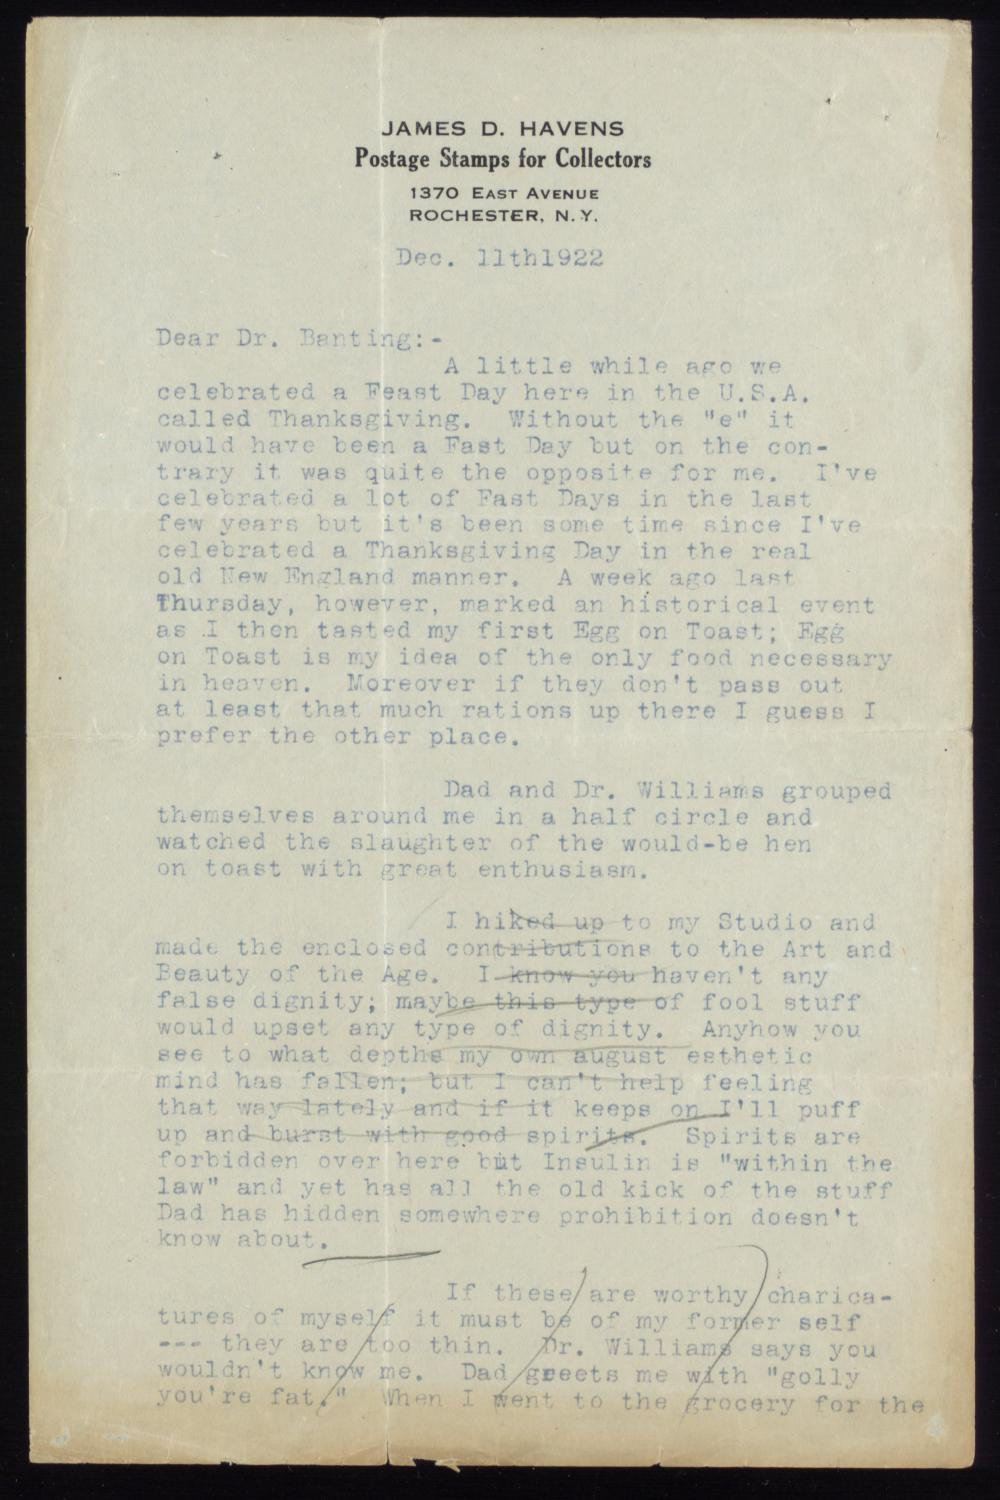
\includegraphics [width=5in]{thanksgivinghavens}
  \caption{Letter from James Havens to Dr. Banting (December 11, 1922)}
  \label{fig: Thanksgiving Letter}
\end{figure}

\begin{figure}[H]
\centering
  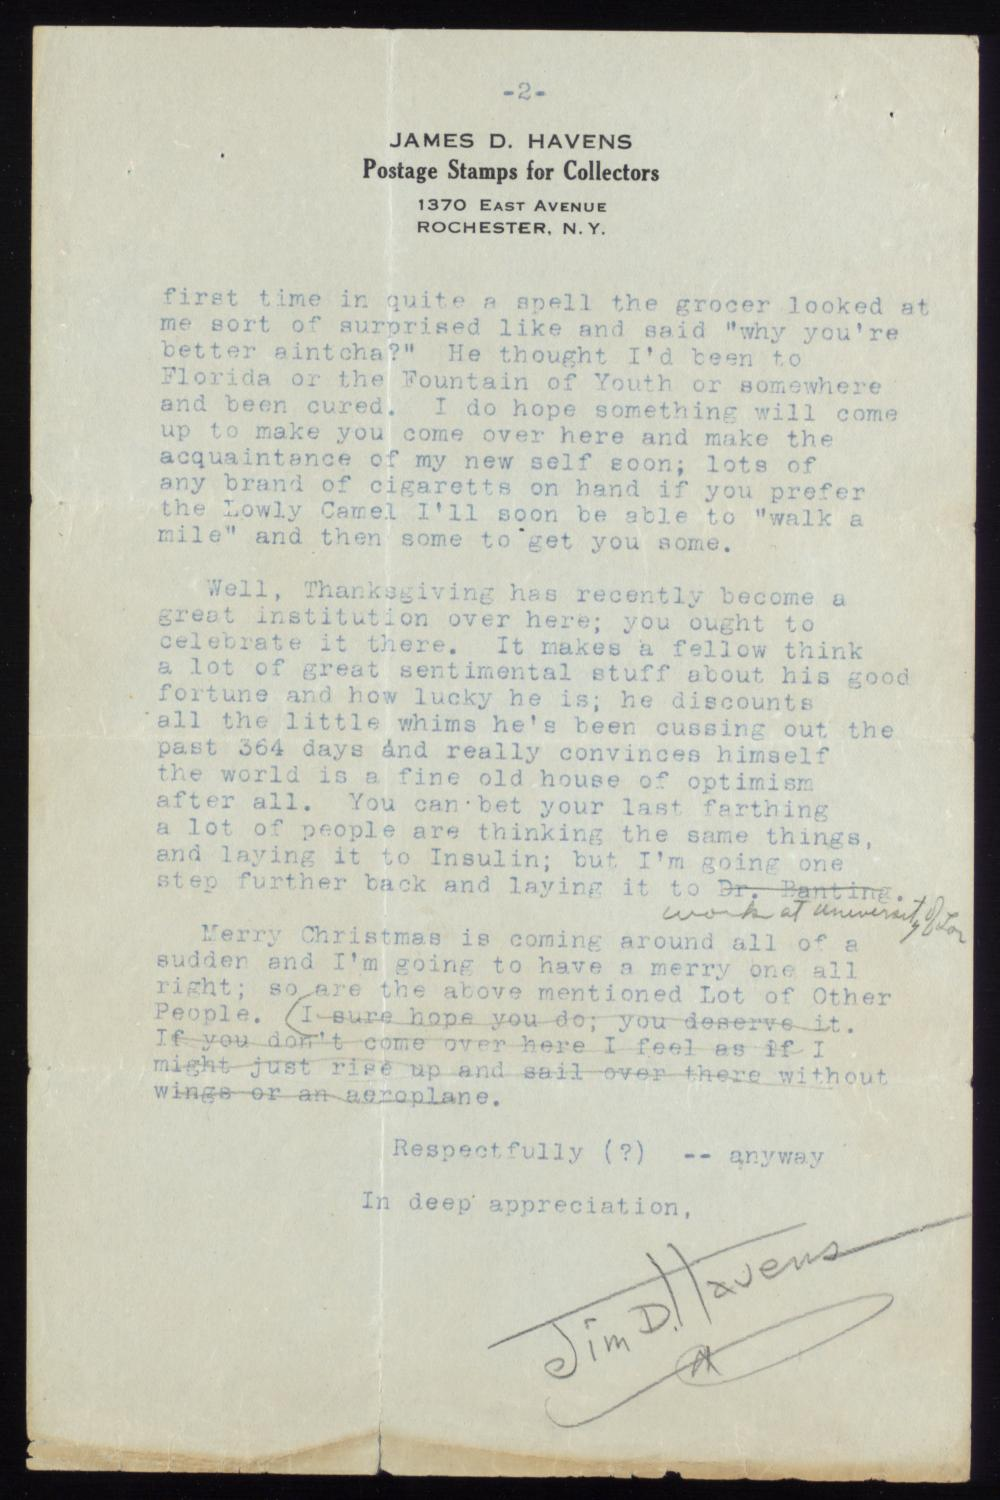
\includegraphics [width=5in]{thankshavep2}
  \caption{Letter from James Havens to Dr. Banting P. 2 (December 11, 1922)}
  \label{fig: Thanksgiving Letter P. 2}
\end{figure}

The following primary source material is from the Bating Collection (MS COll 76) in Fisher Rare Book Library at the University of Toronto as well as the University of Toronto Archives. 
On Decemeber 15, 1922, one of Dr. Josilin's patients, Richard Witner, sent a letter to Banting from Rock Hill, South Carolina, which expresses gratitude for the impact insulin has had on his life:
``As long as I live I'll think of you with the greatest gratitude. You have saved the lives of so many and given happiness to diabeteics all of the world.''
Here, Witner does not merely acknowledge the saving of lives in a medical or physical sense, but also recognizes the impact on the emotional lives of PWD the world over. 

Helen Zualey, another of Joslin's patients, wrote to Banting from her Portland, Maine home on December 14, 1922. She wrote, ``Thru your wonderful discovery of insulin [I] am able to enjoy one of the best things I have been deprived of, namely a \underline{good diet}. I feel like a different girl.'' 
Here Helen brings up one of the emotional relationships regarding diabetes, that is, the human relationship to food. 

Richard Lester of Savannah, Georgia wrote to Dr. Banting on January 26, 1923 to describe his daughter's state before using insulin:
``In the meantime, the child who is of a very happy nature, and extraordinarily bright, became dazed, and took no interest in anything.''
Richard goes on to describe his daughter after being treated with insulin: ``the patient was sitting up in bed singing and playing with her toys. In 48 hours she was up. While still emaciated, she is apparently herself.'' 

Elise Downing Spinar write to Bating about her husband on June 25, 1924. She described his state:
``Until about 2 months ago he has carried on fairly well despite a very active life. Then he had a complete breakdown, lost weight rapidly and found he was suffering from acetone poinsoning.'' Elise's husband went to Duff House in Scotland for treatment and ``now he finds that with injecting insulin twice a day that he is able to absolutely control the acetone and sugar, and from a nervous wreck he seems to be strong, vigorous and altogether a different man.''
This letter illustrates how one becomes a ``nervous wreck'' when living with diabetes. 

Greta Rudberg of Sweden sent a letter written on September 15, 1925 to Banting describes her son's state after using insulin:
``Not only is his life thereby saved but he is as well, happy and full of life as any sound child.''
She makes a point to go beyond gratitude for saving his life and speaks to the quality of his emotional life. 

Ruth Henry of New York (January 6, 1928) wrote to Banting, ``I would venture to tell you of one rich and joyous life that had returned from the Valley of the Shadow as a result of your work. Now here I am, a normal happy and I even hope useful individual in the strenuous life a rural parsonage, glad to be alive and grateful to you.'' 

In the late 1920s, after the wider spread and availability of insulin, there were some who began to notice various concerns. John Comyn of Kent, England wrote, ``I do not wish to seem ungrateful for I am most grateful for what you have already done in the research line; but injections at the rate of 3 per day every day of one's life become wearying and depressing at times'' (December 1, 1929). 

Alice Faulkner of Selma, Alabama wrote to Banting on January 2, 1929 about her daughter with diabetes, `` The doctors here are more afraid of the harm that the insulin will do than they are aware of the good it does.'' This shows a glimpse into the emotional risk taken on by Physicians administering insulin for the first time, perhaps fearful of causing hypoglycemia. Alice described her daughter after the use of insulin, ``In fact, she has more life and `pep' than anyone I know of.'' 


\begin{figure}[H]
\centering
  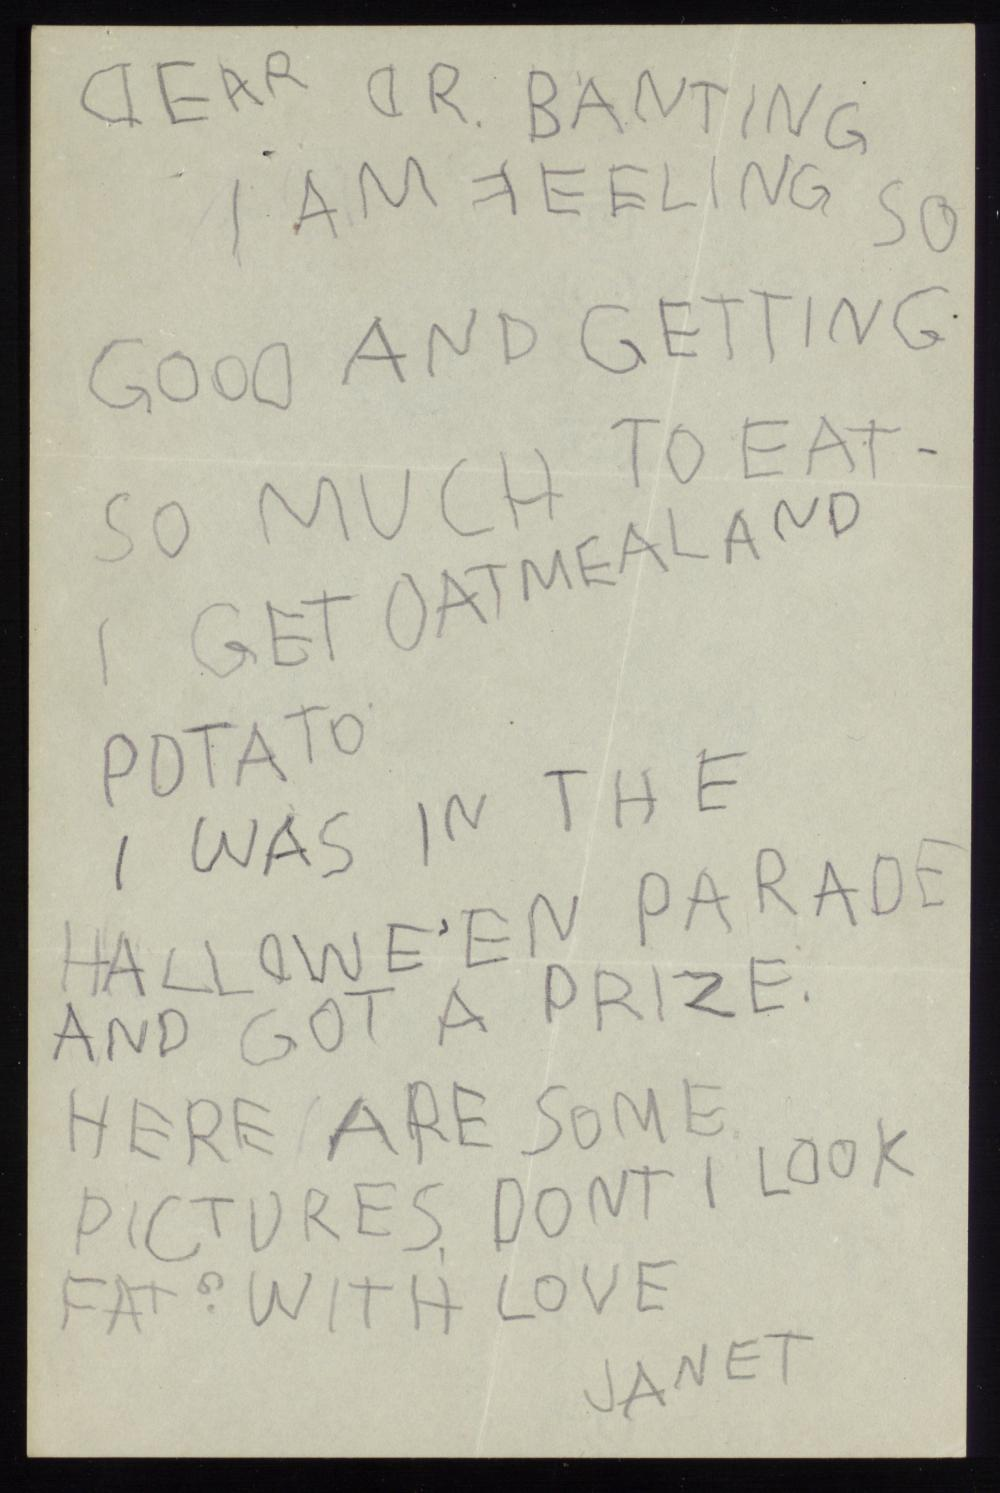
\includegraphics [width=5.5in]{banting_fat}
  \caption{Letter to Dr. Banting from Janet}
  \label{fig:Letter from Janet}
\end{figure}

The introduction of insulin into medicine was by a group of men at the University of Toronto, who then sent the recipes to a group of men at Eli Lilly Corp for improvemnet, production and distribution. 

In the following letter, Dr. Woodyatt writes to Dr. MacLeod to update him on the improvement of his patients with diabetes. One patient stands out to him among the rest:
\begin{quote} \singlespacing
We have one man appeared to be incapable of burning more than 46 g. of glucose, whose power to burn has increased by 33 g. for each cc. of this same preparation. I think that this striking improvement is due in part to the tremendous relief of mental depression that it was for this man to find that his condition was not hopeless and that he could again take a comfortable diet... Diabetics are extremely sensitive to psychic influences, and I have seen in the past many cases whose actual severity varied tremendously in response to such things\footnote{Letter to Dr. MacLeod, October 4 1922. University of Toronto Archives, A1982-0001, Box 15, Folder 4}\end{quote}. 

\begin{figure}[H]
\centering
  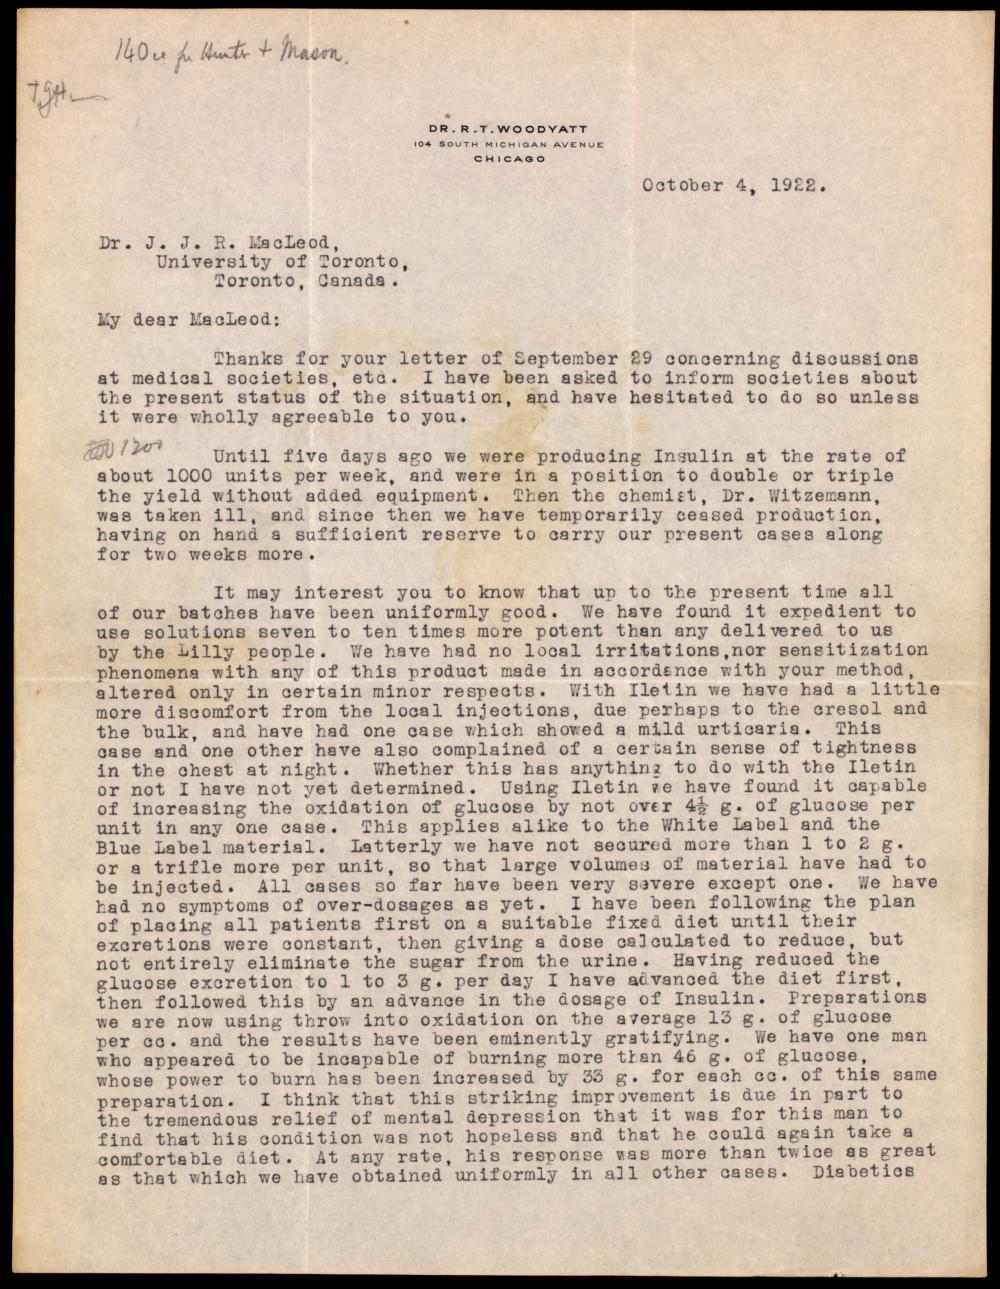
\includegraphics [width=5in]{mental_man}
  \caption{Letter from Dr. R.T Woodyatt to Dr. MacLeod (October 4, 1922)}
  \label{fig: Letter from Dr. R. T. Woodyatt to Dr. MacLeod P. 1}
\end{figure}

\begin{figure}[H]
\centering
  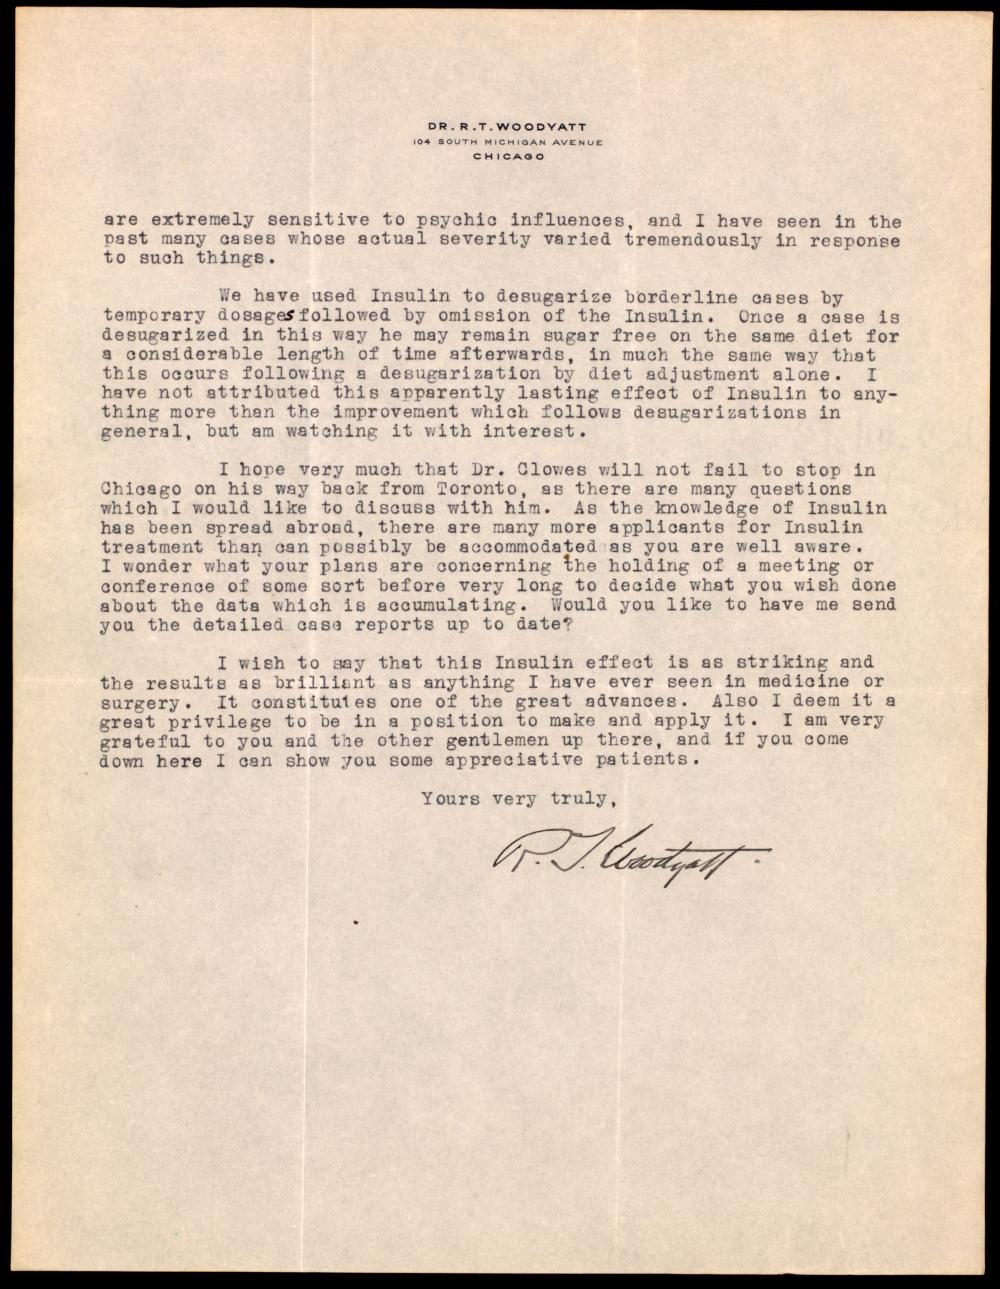
\includegraphics [width=5in]{mental_manp2}
  \caption{Letter from Dr. R.T Woodyatt to Dr. MacLeod P. 2 (October 4, 1922)}
  \label{fig: Letter from Dr. R. T. Woodyatt to Dr. MacLeod P. 2}
\end{figure}
%\newpage
%\section{Major Players}
%It might be of use to introduce researchers and doctors who have been particularly visible in the world of diabetes focused medicine as well as historians of diabetes. 
%Thomas Willis
%G. E. Daniels
%Papaspyros
%Charles Best
%Frederick Banting
%Joslin
%George Burch
%Collip
%McLeod
%White, P. 

%\subsection{Lists}

\newpage
\singlespacing
\bibliographystyle{apa}
\bibliography{dissertation_bibliography}

\end{document}